\begin{figure}[h]
\centering

% --- Top row: per-task probing targets (image + label tightly coupled per panel) ---
\begin{minipage}[b]{0.235\columnwidth}
	\centering
	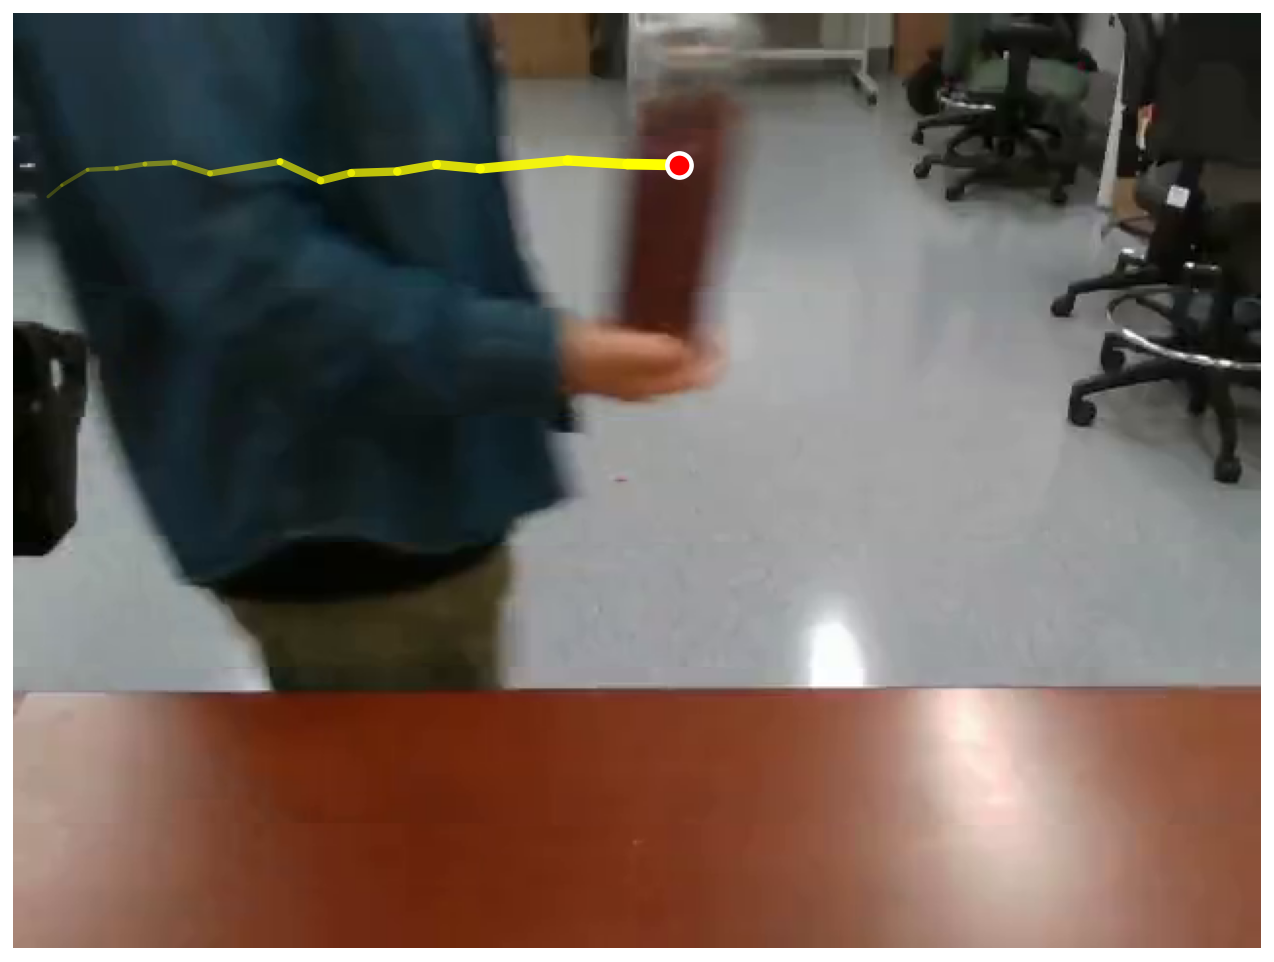
\includegraphics[width=\linewidth]{2026-corl-unveil-template/figures/velocity_handover.png}\\
	{\small Bottle Handover}
\end{minipage}\hfill
\begin{minipage}[b]{0.235\columnwidth}
	\centering
	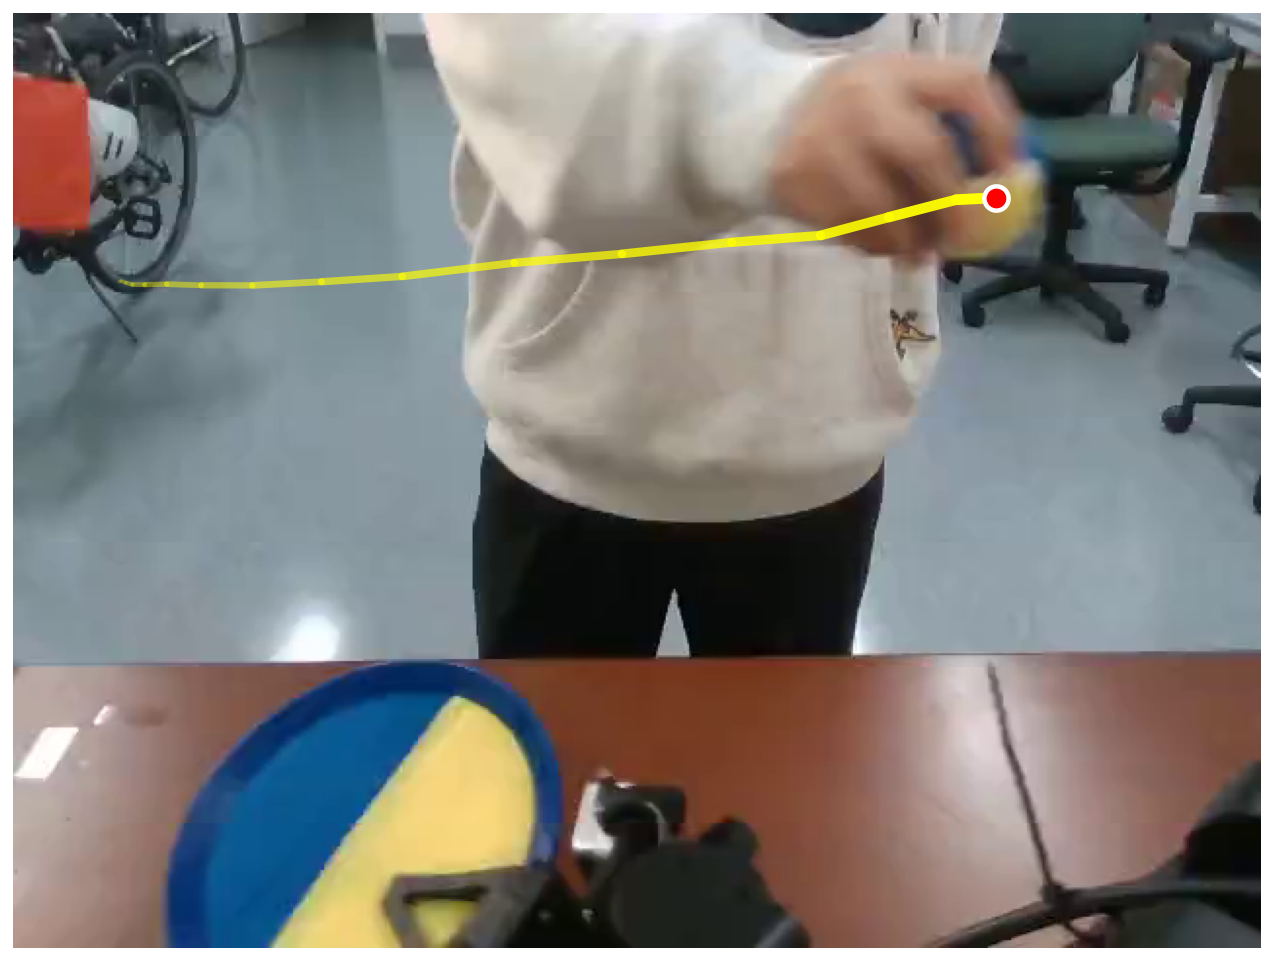
\includegraphics[width=\linewidth]{2026-corl-unveil-template/figures/velocity_drop.png}\\
	{\small Drop Catch}
\end{minipage}\hfill
\begin{minipage}[b]{0.235\columnwidth}
	\centering
	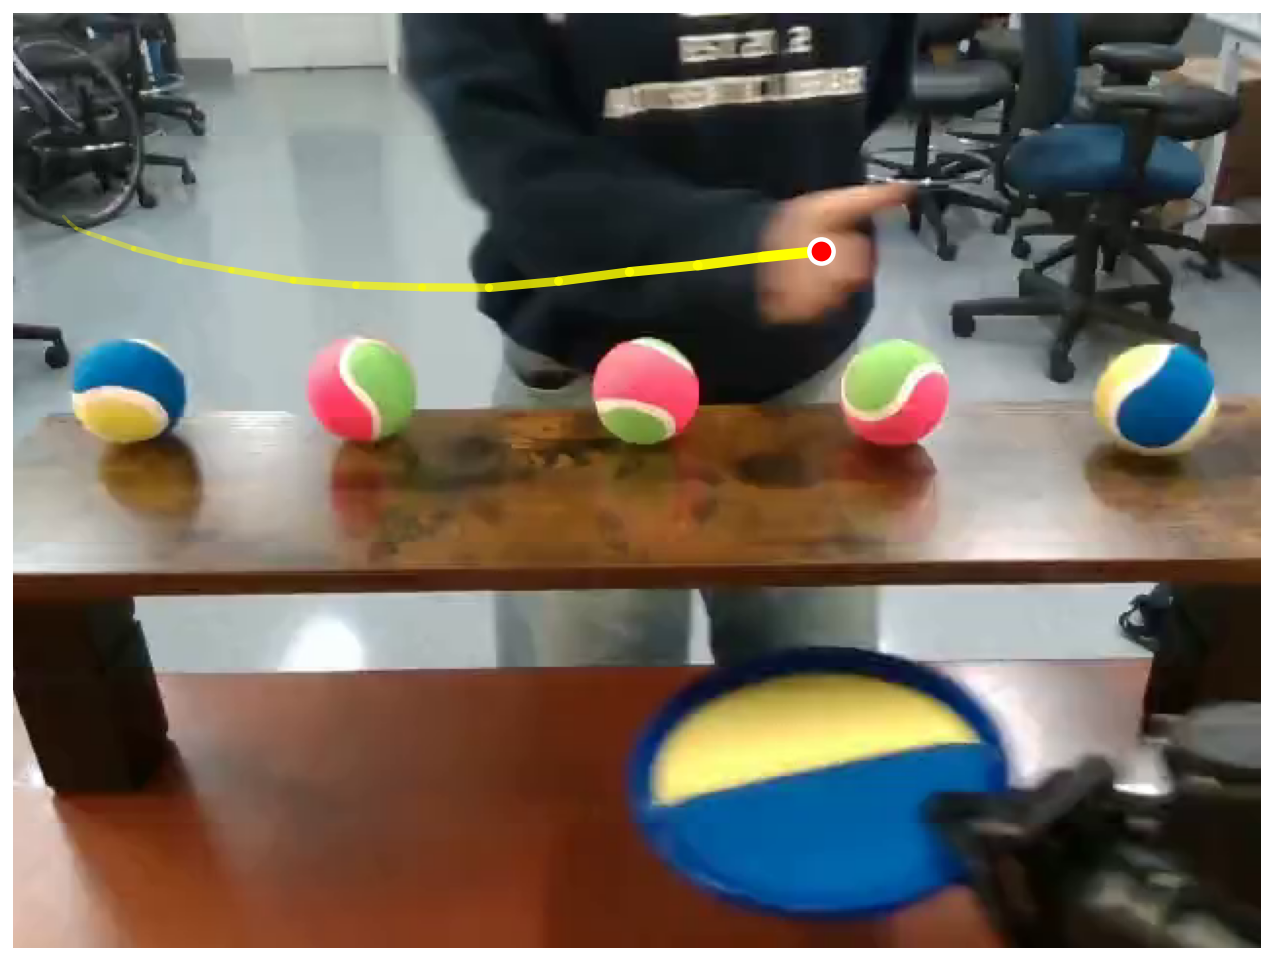
\includegraphics[width=\linewidth]{2026-corl-unveil-template/figures/velocity_flick.png}\\
	{\small Flick Catch}
\end{minipage}\hfill
\begin{minipage}[b]{0.235\columnwidth}
	\centering
	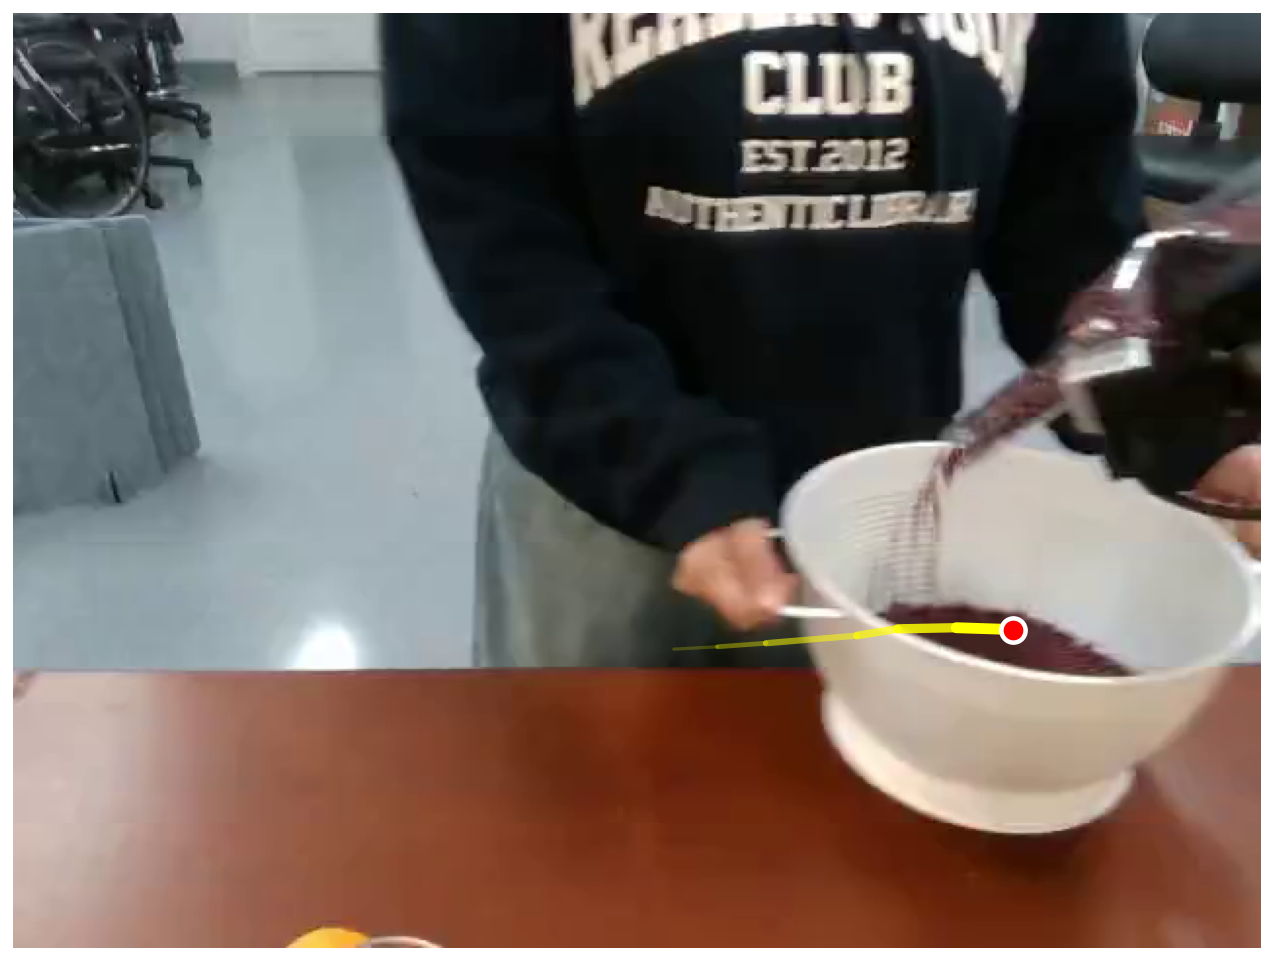
\includegraphics[width=\linewidth]{2026-corl-unveil-template/figures/velocity_pour.png}\\
	{\small Wine Pour}
\end{minipage}

\vspace{8pt}

% --- Bottom: probe results ---
\small
\begin{tabular}{lccccc}
\toprule
\textbf{Initialization for \TEMPOMOT} & \textbf{Bottle Handover} & \textbf{Drop Catch} & \textbf{Flick Catch} & \textbf{Wine Pour} & \textbf{Average} \\
\midrule
% Random                                & -0.01 & 0.00 & 0.00 & 0.00 & 0.00 \\
Object Position                          & 0.24  & 0.03 & 0.03 & 0.02 & 0.08 \\
VideoLaVIT~\cite{videolavit}             & 0.45  & 0.25 & 0.28 & 0.36 & 0.34 \\
Reducio~\cite{reducio}                   & 0.50  & 0.36 & 0.38 & 0.32 & 0.39 \\
SAM~2~\cite{sam2}                        & 0.58  & 0.37 & 0.50 & 0.39 & 0.46 \\
VidTwin~\cite{vidtwin}                   & 0.59  & 0.44 & 0.43 & 0.45 & 0.48 \\
\bottomrule
\end{tabular}

\caption{\textbf{Linear probe of candidate initializations for \TEMPOMOT.} \emph{Top:} one example frame per task showing the object of interest (red dot) and its recent trajectory (yellow line); the pixel-space velocity of this object is the regression target the linear probe must predict. \emph{Bottom:} per-task velocity $R^2$ for each candidate initialization, along with the average. Higher is better; the raw object-position baseline ($R^2=0.08$ on average) cannot recover velocity from a single position, while every learned motion encoder does so substantially better.}
\label{fig:ball_velocity_probe}
\end{figure}
